\begin{appendices}

\chapter{Example Manual Annotations} \label{appendix:example_annotations}

\begin{figure}[!tbp]
	\centering
	\vspace{5mm}
	\begin{subfigure}[t]{0.47\textwidth}
		\centering
    	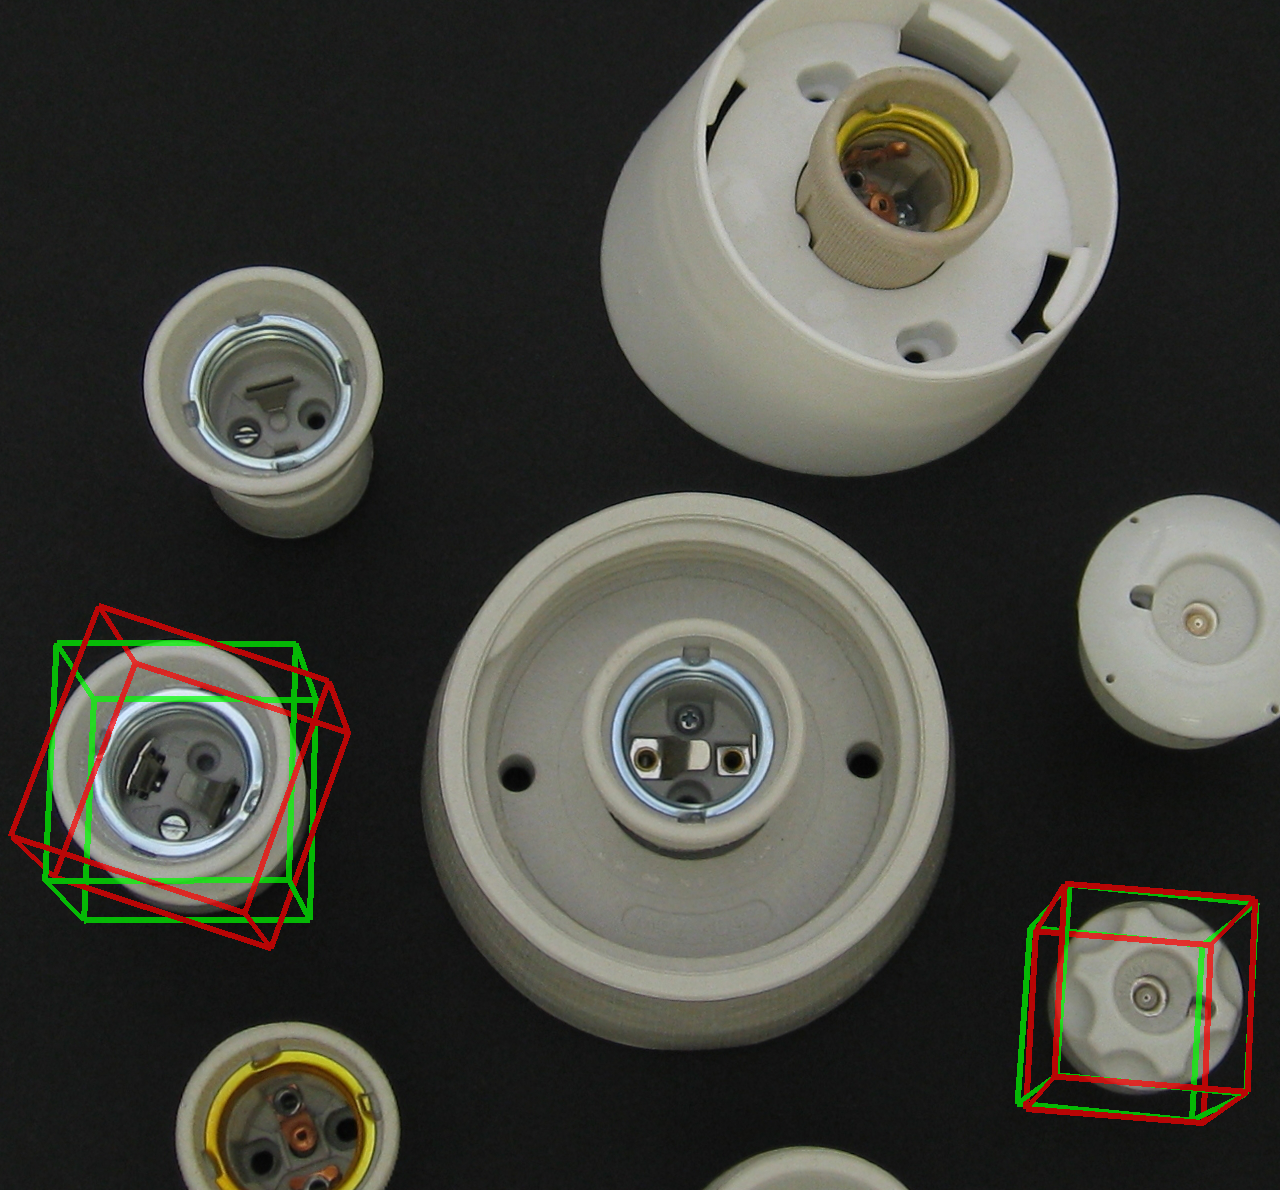
\includegraphics[width=\linewidth]{6dpat_exp_0000}
    	\caption{Image 0000.jpg.}
	\end{subfigure}
	\hfill
	\begin{subfigure}[t]{0.47\textwidth}
		\centering
    	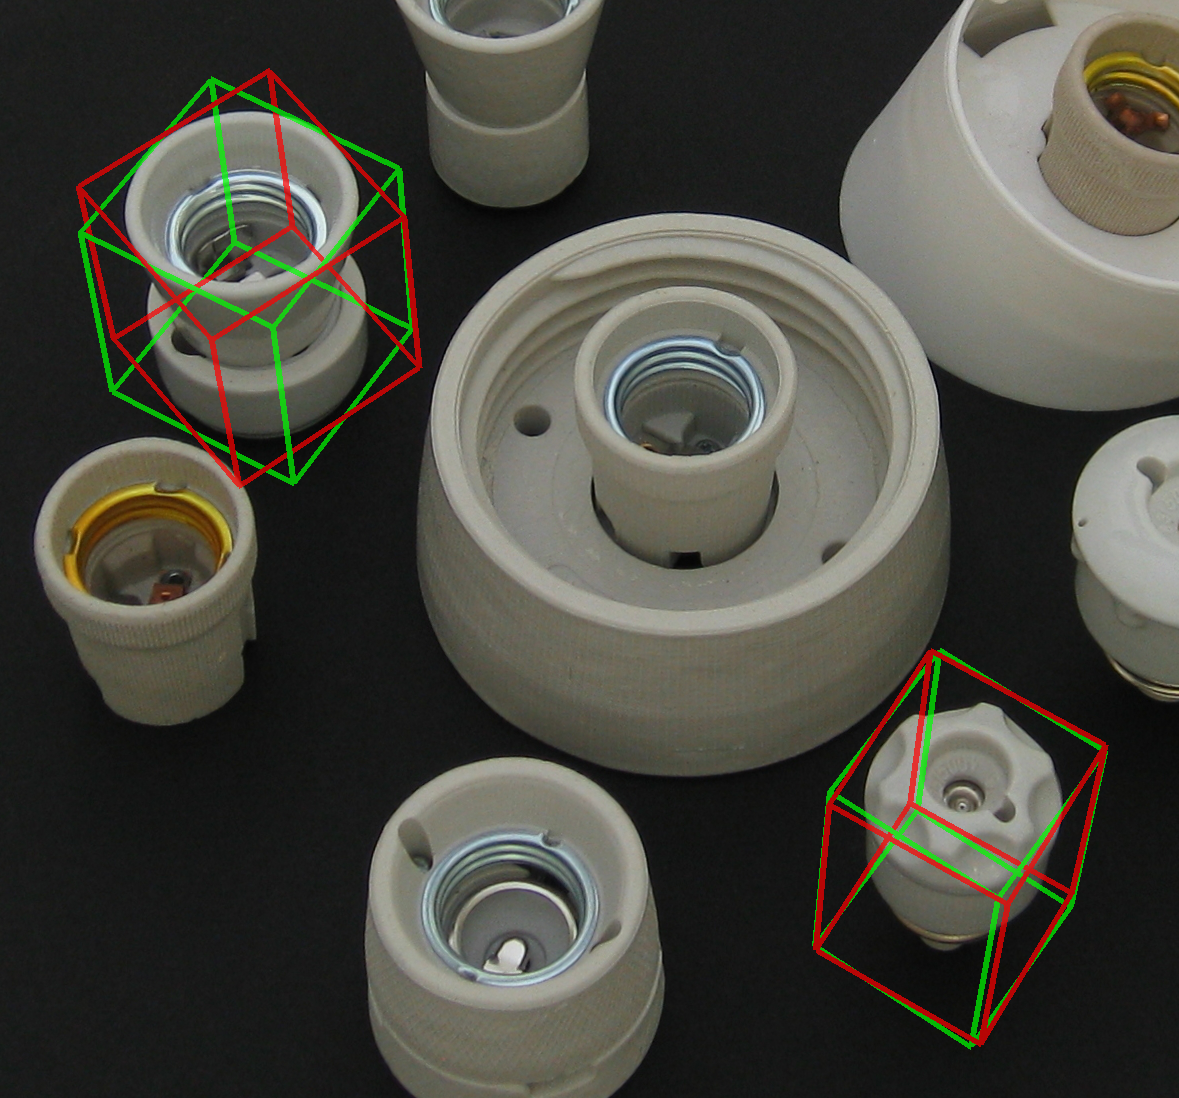
\includegraphics[width=\linewidth]{6dpat_exp_0150}
    	\caption{Image 0150.jpg.}
	\end{subfigure}
	\par\bigskip
	\begin{subfigure}[t]{0.47\textwidth}
		\centering
    	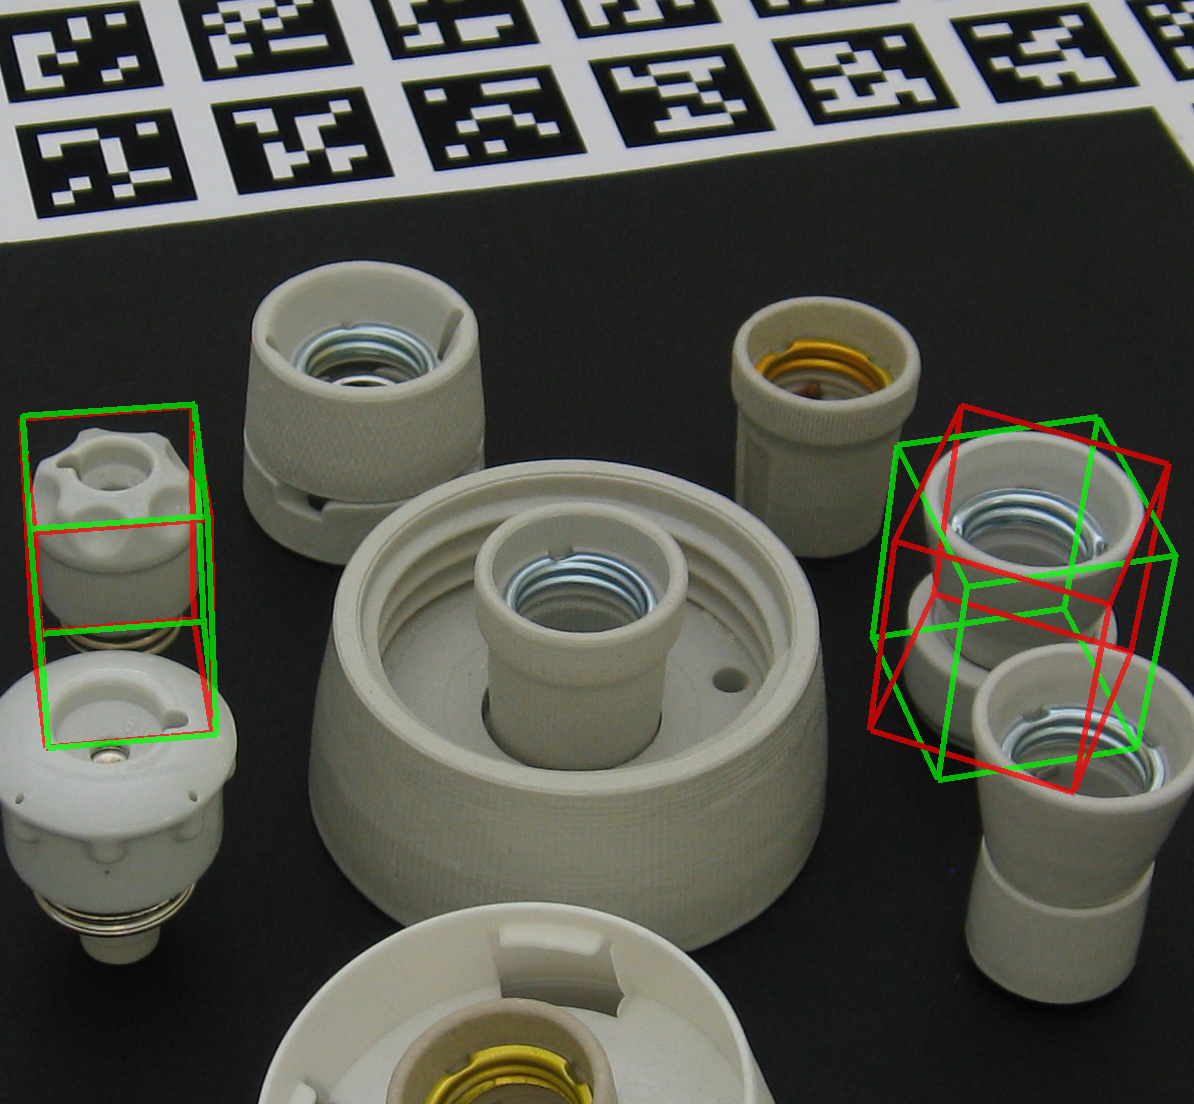
\includegraphics[width=\linewidth]{6dpat_exp_0250}
    	\caption{Image 0250.jpg.}
	\end{subfigure}
	\hfill
	\begin{subfigure}[t]{0.47\textwidth}
		\centering
    	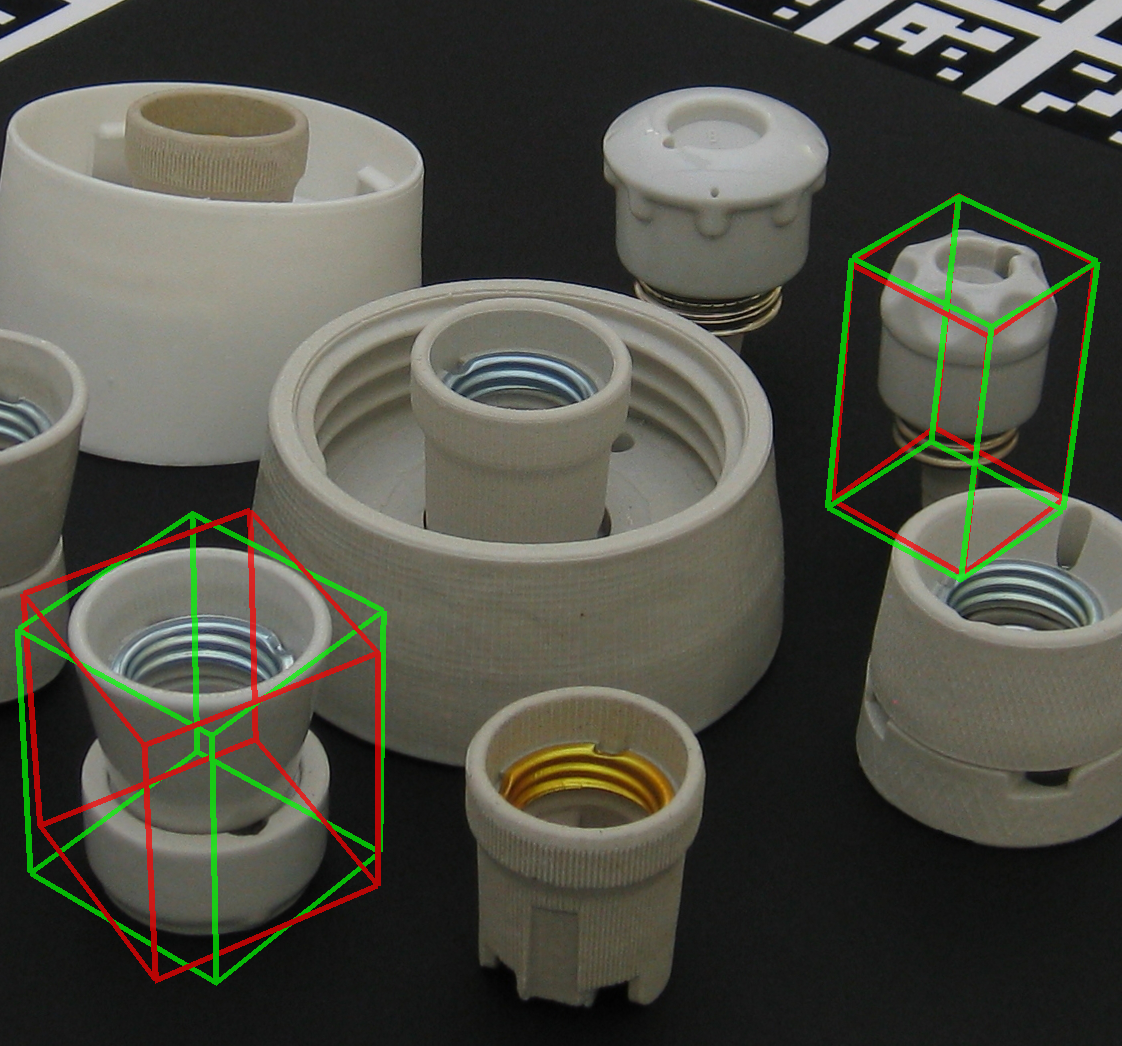
\includegraphics[width=\linewidth]{6dpat_exp_0350}
    	\caption{Image 0350.jpg.}
	\end{subfigure}
	\par\bigskip
	\begin{subfigure}[t]{0.47\textwidth}
		\centering
    	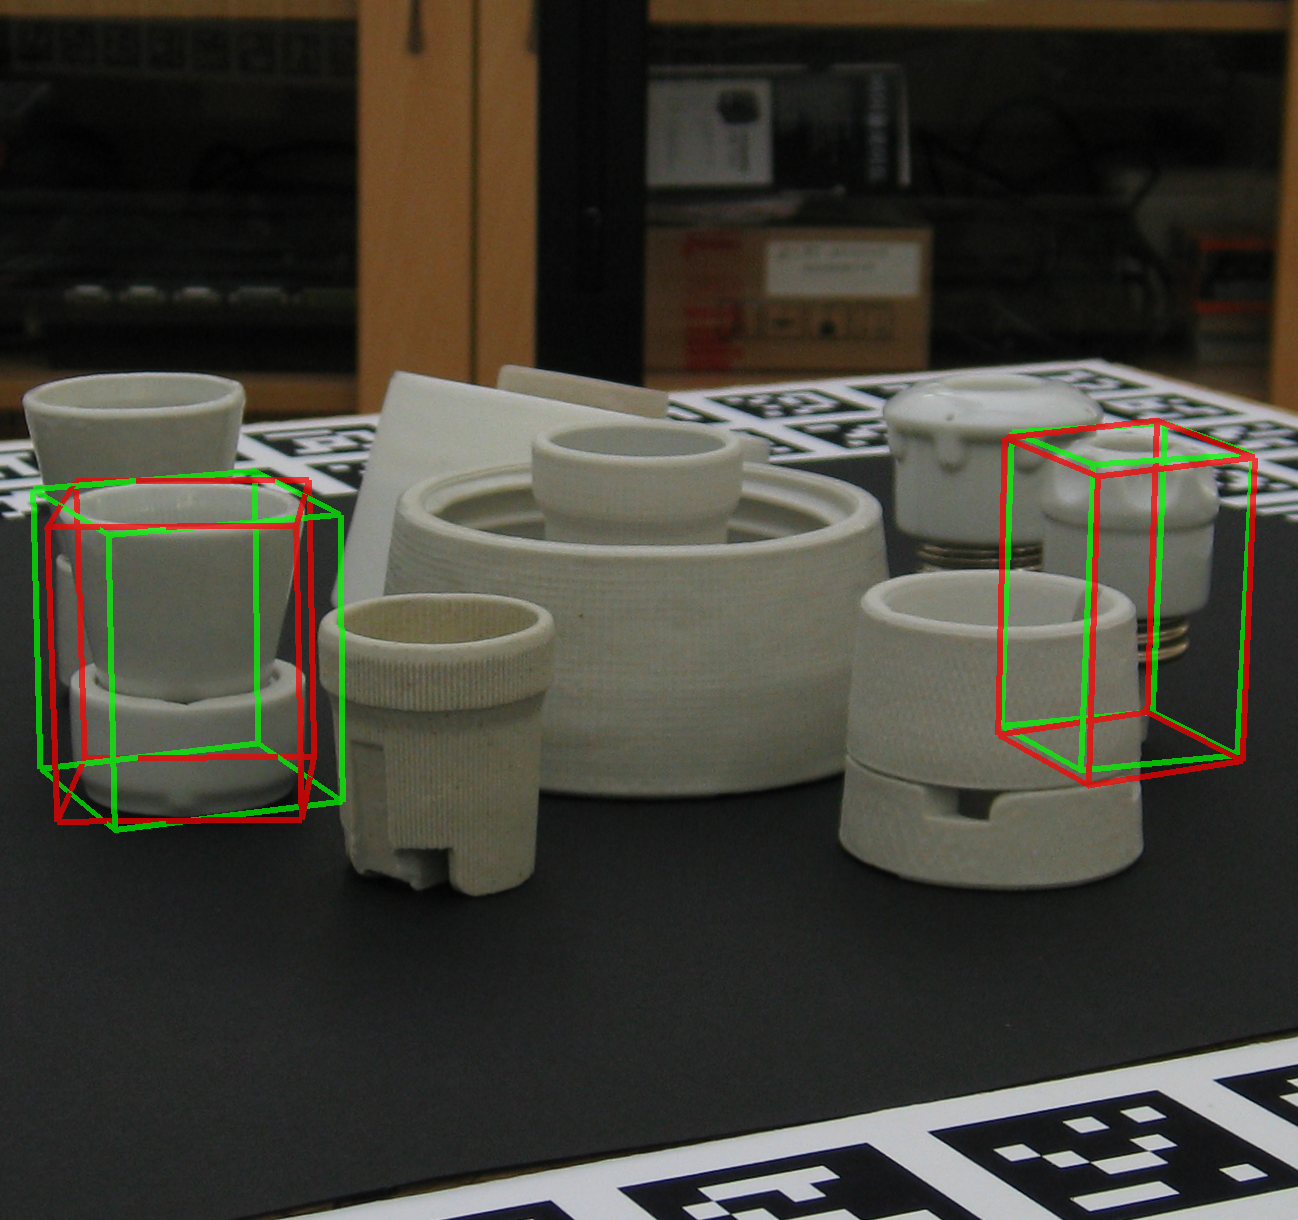
\includegraphics[width=\linewidth]{6dpat_exp_0500}
    	\caption{Image 0500.jpg.}
	\end{subfigure}
	\caption{Example images from test scene 7 of the T-Less dataset with the poses recovered using \ac{6dpat}. The images are cropped to the relevant area.}
\end{figure} 

\chapter{Network Architectures} \label{appendix:network_architectures}

\begin{figure}[!tbp]
	\centering
    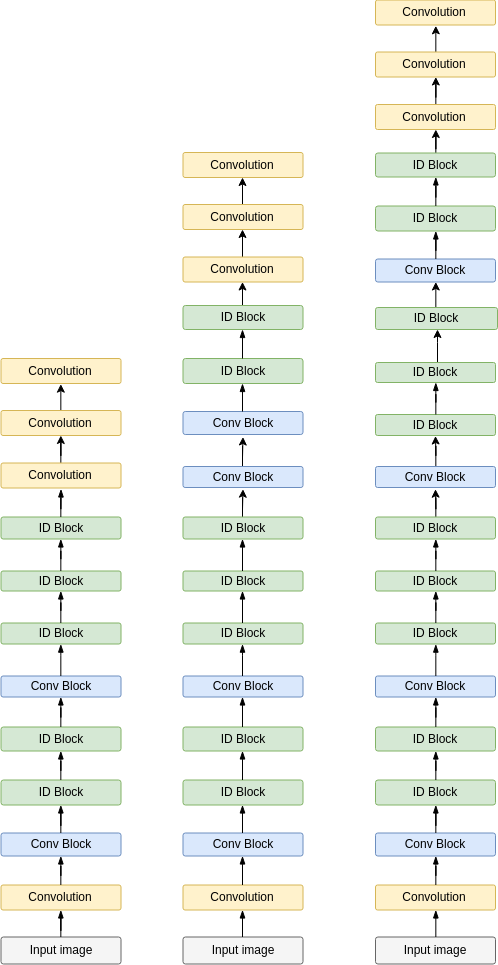
\includegraphics[width=0.7\linewidth]{network_architecture_comparison}
    \caption{The different architectures used in this work. Architectures 1 and 3 use the leftmost structure with a total of 23 convolutional layers. We constructed architecture 2 using the layout in the middle with 35 layers. Architectures 4, 5 and 6 use the 50 layers structured as shown on the right, although architectures 4 and 6 employ dropout layers with different frequencies after each block and omit the batchnormalization layers. We omitted the batchnormalization layers in the other to structures for displaying purposes.}
    \label{fig:network_architecture_comparison}
\end{figure} 

\chapter{Experiments}

\begin{figure}[!tbp]
	\begin{subfigure}[t]{0.4\textwidth}
			\begin{tikzpicture}[scale=0.95]
  				\begin{axis}[cycle list name=tb, 
                 grid=both,
                 grid style={solid,gray!30!white},
                 axis lines=middle,
    			 xmin = 0,
    			 xmax = 50,
    			 ymin = 0,
    			 ymax = 15,
                 xlabel={step},
                 ylabel={value},
                 x label style={at={(axis description cs:0.5,-0.1)},anchor=north},
                 y label style={at={(axis description cs:-0.1,.5)},rotate=90,anchor=south},]
      			\addplot[smooth,tb_color_1] table [x=Step, y=Value, col sep=comma] {experiments/model1/exp1_adam_l1/train_loss.csv};
      			\addplot[smooth,tb_color_2] table [x=Step, y=Value, col sep=comma] {experiments/model1/exp1_adam_l2/train_loss.csv};
      			\addlegendentry{L1}
				\addlegendentry{L2}
    			\end{axis}
			\end{tikzpicture}
		\caption{Training losses.}
	\end{subfigure}
	\hspace{15mm}
	\begin{subfigure}[t]{0.4\textwidth}
			\begin{tikzpicture}[scale=0.95]
  				\begin{axis}[cycle list name=tb, 
                 grid=both,
                 grid style={solid,gray!30!white},
                 axis lines=middle,
    			 xmin = 0,
    			 xmax = 50,
    			 ymin = 0,
    			 ymax = 15,
                 xlabel={step},
                 ylabel={value},
                 x label style={at={(axis description cs:0.5,-0.1)},anchor=north},
                 y label style={at={(axis description cs:-0.1,.5)},rotate=90,anchor=south},]
      			\addplot[smooth,tb_color_1] table [x=Step, y=Value, col sep=comma] {experiments/model1/exp1_adam_l1/val_loss.csv};
      			\addplot[smooth,tb_color_2] table [x=Step, y=Value, col sep=comma] {experiments/model1/exp1_adam_l2/val_loss.csv};
      			\addlegendentry{L1}
				\addlegendentry{L2}
    			\end{axis}
			\end{tikzpicture}
		\caption{Validation losses.}
	\end{subfigure}
	\caption{Training and validation losses of the L1 and L2 loss of training architecture 1. The plot is cropped on the $y$-axis to enhance the differences.}
	\label{fig:experiments_l1_l2_loss}
\end{figure} 

\begin{figure}[!tbp]
	\centering
	\vspace{5mm}
	\begin{subfigure}[t]{0.47\textwidth}
		\centering
    	\includegraphics[width=\linewidth]{experiments/model2/0045_bounding_boxes}
    	\caption{Image 0045.jpg, pose recovered using architecture 2.}
	\end{subfigure}
	\hfill
	\begin{subfigure}[t]{0.47\textwidth}
		\centering
    	\includegraphics[width=\linewidth]{experiments/model2/0438_bounding_boxes}
    	\caption{Image 0438.jpg, pose recovered using architecture 2.}
	\end{subfigure}
	\par\bigskip
	\begin{subfigure}[t]{0.47\textwidth}
		\centering
    	\includegraphics[width=\linewidth]{experiments/model3/0045_bounding_boxes}
    	\caption{Image 0045.jpg, pose recovered using architecture 3.}
	\end{subfigure}
	\hfill
	\begin{subfigure}[t]{0.47\textwidth}
		\centering
    	\includegraphics[width=\linewidth]{experiments/model3/0438_bounding_boxes}
    	\caption{Image 0438.jpg, pose recovered using architecture 3.}
	\end{subfigure}
	\par\bigskip
	\begin{subfigure}[t]{0.47\textwidth}
		\centering
    	\includegraphics[width=\linewidth]{experiments/model5/0045_bounding_boxes}
    	\caption{Image 0045.jpg, pose recovered using architecture 5.}
	\end{subfigure}
	\hfill
	\begin{subfigure}[t]{0.47\textwidth}
		\centering
    	\includegraphics[width=\linewidth]{experiments/model5/0438_bounding_boxes}
    	\caption{Image 0438.jpg, pose recovered using architecture 5.}
	\end{subfigure}
	\caption{Example images from test scene 7 with rendered poses recovered by the architecture mentioned in the image caption.}
	\label{fig:appendix_architecture_comparison_example_frames}
\end{figure}

\begin{figure}[!tbp]
	\begin{subfigure}[t]{0.4\textwidth}
			\begin{tikzpicture}[scale=0.95]
  				\begin{axis}[cycle list name=tb, 
                 grid=both,
                 grid style={solid,gray!30!white},
                 axis lines=middle,
                 xlabel={epoch},
                 xmax = 100,
    			 ymax = 8,
                 ylabel={loss},
                 x label style={at={(axis description cs:0.5,-0.1)},anchor=north},
                 y label style={at={(axis description cs:-0.1,.5)},rotate=90,anchor=south},]
      			\addplot[line width=2pt,dotted,tb_color_1] table [x=Step, y=Value, col sep=comma] {experiments/model5/exp7_25/train_loss.csv};
      			\addplot[line width=2pt,dotted,tb_color_2] table [x=Step, y=Value, col sep=comma] {experiments/model5/exp7_50/train_loss.csv};
      			\addplot[line width=2pt,dotted,tb_color_3] table [x=Step, y=Value, col sep=comma] {experiments/model5/exp7_100/train_loss.csv};
      			\addplot[line width=2pt,dotted,tb_color_4] table [x=Step, y=Value, col sep=comma] {experiments/model5/exp7_250/train_loss.csv};
      			\addplot[line width=1pt,smooth,tb_color_5] table [x=Step, y=Value, col sep=comma] {experiments/model5/exp3/train_loss.csv};
      			\addplot[line width=1pt,smooth,tb_color_6] table [x=Step, y=Value, col sep=comma] {experiments/model5/exp4/train_loss.csv};
      			\addplot[line width=1pt,smooth,tb_color_7] table [x=Step, y=Value, col sep=comma] {experiments/model5/exp5/train_loss.csv};
      			\addplot[line width=1pt,smooth,tb_color_8] table [x=Step, y=Value, col sep=comma] {experiments/model5/exp6/train_loss.csv};
				\addlegendentry{25 [inc 70/30]}
				\addlegendentry{50 [inc 70/30]}
				\addlegendentry{100 [inc 70/30]}
				\addlegendentry{250 [inc 70/30]}
				\addlegendentry{250}
				\addlegendentry{100}
				\addlegendentry{50}
				\addlegendentry{25}
    			\end{axis}
			\end{tikzpicture}
		\caption{Training losses.}
	\end{subfigure}
	\hspace{15mm}
	\begin{subfigure}[t]{0.4\textwidth}
			\begin{tikzpicture}[scale=0.95]
  				\begin{axis}[cycle list name=tb, 
                 grid=both,
                 grid style={solid,gray!30!white},
                 axis lines=middle,
                 xlabel={epoch},
    			 xmax = 100,
    			 ymax = 20,
                 ylabel={loss},
                 x label style={at={(axis description cs:0.5,-0.1)},anchor=north},
                 y label style={at={(axis description cs:-0.1,.5)},rotate=90,anchor=south},]
      			\addplot[line width=2pt,dotted,tb_color_1] table [x=Step, y=Value, col sep=comma] {experiments/model5/exp7_25/val_loss.csv};
      			\addplot[line width=2pt,dotted,tb_color_2] table [x=Step, y=Value, col sep=comma] {experiments/model5/exp7_50/val_loss.csv};
      			\addplot[line width=2pt,dotted,tb_color_3] table [x=Step, y=Value, col sep=comma] {experiments/model5/exp7_100/val_loss.csv};
      			\addplot[line width=2pt,dotted,tb_color_4] table [x=Step, y=Value, col sep=comma] {experiments/model5/exp7_250/val_loss.csv};
      			\addplot[line width=1pt,smooth,tb_color_5] table [x=Step, y=Value, col sep=comma] {experiments/model5/exp3/val_loss.csv};
      			\addplot[line width=1pt,smooth,tb_color_6] table [x=Step, y=Value, col sep=comma] {experiments/model5/exp4/val_loss.csv};
      			\addplot[line width=1pt,smooth,tb_color_7] table [x=Step, y=Value, col sep=comma] {experiments/model5/exp5/val_loss.csv};
      			\addplot[line width=1pt,smooth,tb_color_8] table [x=Step, y=Value, col sep=comma] {experiments/model5/exp6/val_loss.csv};
    			\end{axis}
			\end{tikzpicture}
		\caption{Validation losses.}
	\end{subfigure}
	
	\begin{subfigure}[t]{0.4\textwidth}
			\begin{tikzpicture}[scale=0.95]
  				\begin{axis}[cycle list name=tb, 
                 grid=both,
                 grid style={solid,gray!30!white},
                 axis lines=middle,
                 xlabel={epoch},
                 xmax = 50,
    			 ymax = 8,
                 ylabel={loss},
                 x label style={at={(axis description cs:0.5,-0.1)},anchor=north},
                 y label style={at={(axis description cs:-0.1,.5)},rotate=90,anchor=south},]
      			\addplot[line width=2pt,dotted,tb_color_1] table [x=Step, y=Value, col sep=comma] {experiments/model5/exp8_25/train_loss.csv};
      			\addplot[line width=2pt,dotted,tb_color_2] table [x=Step, y=Value, col sep=comma] {experiments/model5/exp8_50/train_loss.csv};
      			\addplot[line width=2pt,dotted,tb_color_3] table [x=Step, y=Value, col sep=comma] {experiments/model5/exp8_100/train_loss.csv};
      			\addplot[line width=2pt,dotted,tb_color_4] table [x=Step, y=Value, col sep=comma] {experiments/model5/exp8_250/train_loss.csv};
      			\addplot[line width=1pt,smooth,tb_color_5] table [x=Step, y=Value, col sep=comma] {experiments/model5/exp3/train_loss.csv};
      			\addplot[line width=1pt,smooth,tb_color_6] table [x=Step, y=Value, col sep=comma] {experiments/model5/exp4/train_loss.csv};
      			\addplot[line width=1pt,smooth,tb_color_7] table [x=Step, y=Value, col sep=comma] {experiments/model5/exp5/train_loss.csv};
      			\addplot[line width=1pt,smooth,tb_color_8] table [x=Step, y=Value, col sep=comma] {experiments/model5/exp6/train_loss.csv};
				\addlegendentry{25 [inc 90/10]}
				\addlegendentry{50 [inc 90/10]}
				\addlegendentry{100 [inc 90/10]}
				\addlegendentry{250 [inc 90/10]}
				\addlegendentry{250}
				\addlegendentry{100}
				\addlegendentry{50}
				\addlegendentry{25}
    			\end{axis}
			\end{tikzpicture}
		\caption{Training losses.}
	\end{subfigure}
	\hspace{15mm}
	\begin{subfigure}[t]{0.4\textwidth}
			\begin{tikzpicture}[scale=0.95]
  				\begin{axis}[cycle list name=tb, 
                 grid=both,
                 grid style={solid,gray!30!white},
                 axis lines=middle,
                 xlabel={epoch},
    			 xmax = 50,
    			 ymax = 20,
                 ylabel={loss},
                 x label style={at={(axis description cs:0.5,-0.1)},anchor=north},
                 y label style={at={(axis description cs:-0.1,.5)},rotate=90,anchor=south},]
      			\addplot[line width=2pt,dotted,tb_color_1] table [x=Step, y=Value, col sep=comma] {experiments/model5/exp8_25/val_loss.csv};
      			\addplot[line width=2pt,dotted,tb_color_2] table [x=Step, y=Value, col sep=comma] {experiments/model5/exp8_50/val_loss.csv};
      			\addplot[line width=2pt,dotted,tb_color_3] table [x=Step, y=Value, col sep=comma] {experiments/model5/exp8_100/val_loss.csv};
      			\addplot[line width=2pt,dotted,tb_color_4] table [x=Step, y=Value, col sep=comma] {experiments/model5/exp8_250/val_loss.csv};
      			\addplot[line width=1pt,smooth,tb_color_5] table [x=Step, y=Value, col sep=comma] {experiments/model5/exp3/val_loss.csv};
      			\addplot[line width=1pt,smooth,tb_color_6] table [x=Step, y=Value, col sep=comma] {experiments/model5/exp4/val_loss.csv};
      			\addplot[line width=1pt,smooth,tb_color_7] table [x=Step, y=Value, col sep=comma] {experiments/model5/exp5/val_loss.csv};
      			\addplot[line width=1pt,smooth,tb_color_8] table [x=Step, y=Value, col sep=comma] {experiments/model5/exp6/val_loss.csv};
    			\end{axis}
			\end{tikzpicture}
		\caption{Validation losses.}
	\end{subfigure}
	\caption{Training and validation losses of the experiments of training architecture \textbf{5}. The keys are the number of images used in training. \textit{inc} stands for incremental training and the numbers afterwards indicate the split of the training and validation dataset.}
	\label{fig:experiments_online_sratch_loss_arch5}
\end{figure} 

\begin{table}[]
\centering
\begin{tabular}{l||llllll}
Method                   & $e_{\text{coord}}$ & $n_{\text{inlier}}$ & $e_{\text{angle}}$ & $e_{\text{dist}}$ & $e_{\text{pose}}$ & inliers \% \\ \hline \hline
from scratch (25, 70/30)        & 11.5468            & 57.8933                   & 84.3733            & 13.70721           & 23.0772  &    1.33333      \\ \hline
from scratch (50, 70/30)        & 9.2500             & 87.6600                  & 51.2956            & 18.8137           & 23.4164 & 14.0000           \\  \hline 
from scratch (100, 70/30)       & 6.5312             & 151.2266                 & 26.1370             & 40.6087            & 41.934 &    23.3333        \\ \hline 
from scratch (250, 70/30)       & \textbf{4.1992}             & \textbf{332.2933}                 & \textbf{4.7410}             & \textbf{9.2082}            & \textbf{9.4344} & \textbf{62.0000}            \\ \hline \hline
incremental (50, 70/30)  & 12.6562            & 10.6250                   & 97.5586          & 48.7668           & 56.2073 & 6.2500           \\ \hline
incremental (100, 70/30) & 11.3671            & 27.2500                  & 90.8267           & 32.6782           & 38.9909 & 3.1250           \\ \hline
incremental (250, 70/30) & 9.3281             & 68.9375                  & 68.3927           & 34.8104          & 39.7651 &  3.7500         \\ \hline \hline 
incremental (50, 90/20)  & 11.5625            & 5.3333                   & 97.9677           & 131.0969           & 135.8001 & 0.0000          \\ \hline 
incremental (100, 90/10) & 11.9843             & 3.3333                 & 116.4722            & 38.5254          & 46.8544 & 0.0000         \\ \hline
incremental (250, 90/10) & 12.7500            & 15.3333                 & 101.6921            & 107.6326            & 113.3697 & 0.0000         
\end{tabular}
\caption{The evaluation metrics set of the experiments using architecture \textbf{5} on the validation set. The numbers in parentheses are the number of images, followed by the training - validation set split, if specified.}
\label{table:experiments_online_sratch_arch5}
\end{table}

\end{appendices}